\documentclass{if-beamer}

% --------------------------------------------------- %
%                  Presentation info	              %
% --------------------------------------------------- %
\title[Lecture 17]{Lecture 17}
\subtitle{Integration and Differentiation: Unit Overview and Integration with the Trapezoid Rule}
\author{Ashley Gannon}
\date{ISC3313 Fall 2021}
\logo{

\includegraphics[scale=0.08]{figures/FSULogo.png}
}
\subject{Presentation subject}

% --------------------------------------------------- %
%                    Title + Schedule                 %
% --------------------------------------------------- %
\begin{document}

\begin{frame}
  \titlepage
\end{frame}
% --------------------------------------------------- %
%                      Presentation                   %
% --------------------------------------------------- %
\section{Overview}

\begin{frame}
\frametitle{Derivatives and Integration}
\begin{itemize}
	\item In high school or during your first year of college, you were introduced to differential and
	integral calculus.
	\item There you learned techniques to obtain analytical or exact derivatives
	and integrals.
	\item Mathematically, the derivative represents the rate of change of a dependent variable with respect to an independent variable.
	\begin{itemize}
		\item For example, if we are given a function y(t) that
		specifies an object’s position as a function of time, differentiation provides a means to
		determine its velocity, as in
		$$\frac{dy(t)}{dt} = v(t)$$
	\end{itemize}
	\item Integration is the inverse of differentiation.
	\begin{itemize}
		\item Just as differentiation uses differences to quantify an instantaneous
		process, integration involves summing instantaneous information to give a total result over an interval.
		\item if we are provided with velocity as a function of time, integration can be used to determine the distance traveled:
		$$\int_{0}^{t} v(t)dt = y(t)$$ 
	\end{itemize}
	\item In short, think of a derivative as a slope and an integral as a summation.
\end{itemize} 
\end{frame}

\begin{frame}
	\frametitle{Methods we will cover in this unit}
	\begin{itemize}
		\item Integration \\\vspace{4pt}
		\begin{itemize}
			\item Trapezoidal Rule\\\vspace{4pt}
			\item Simpson's 1/3 Rule\\\vspace{4pt}
			\item Simpson's 3/8 Rule\\\vspace{4pt}
			\item Richardson Extrapolation\\\vspace{4pt}
			\item Gauss Quadrature\\\vspace{4pt}
		\end{itemize}
		\item Differentiation\\\vspace{4pt}
		\begin{itemize}
			\item Finite Difference Methods\\\vspace{4pt}
			\item Richardson Extrapolation\\\vspace{4pt}
		\end{itemize}
	\end{itemize}
\end{frame}
\section{Integration}
\begin{frame}
	\frametitle{What is integration}
	\begin{minipage}{0.6\textwidth}
		Mathematically, definite integration is represented by 
		$$I = \int_{a}^{b} f(x)dx$$
		which stands for the integral of the function $f(x)$ with respect to the independent variable $x$ evaluated between the limits $x=a$ and $x=b$. \\\vspace{10pt}
		
		The integral is the summation of $f(x)dx$ over the range of $x=a$ to $x=b$. \\
	\end{minipage}
	\begin{minipage}{0.4\textwidth}
		\begin{figure}
			\centering
			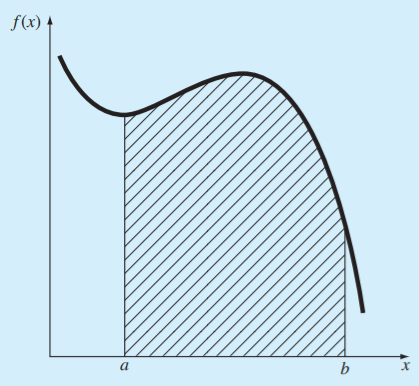
\includegraphics[width=.95\textwidth]{figures/integralplot}
		\end{figure}
	\end{minipage}
	\\\vspace{0.5cm}
	Fun fact: the symbol $\int$ is an elongated letter S to stand for Summa, Latin for sum.
\end{frame}

\begin{frame}[t]
	\frametitle{Integration}
	Recall that the velocity of a free-falling bungee jumper as a function of time can be
	computed as
	$$v(t) = \sqrt{\frac{gm}{c_d}}tanh\left(\sqrt{\frac{gc_d}{m}}t\right) $$
\end{frame}

\begin{frame}[t]
	\frametitle{Integration}
	Recall that the velocity of a free-falling bungee jumper as a function of time can be
	computed as
	$$v(t) = \sqrt{\frac{gm}{c_d}}tanh\left(\sqrt{\frac{gc_d}{m}}t\right) $$
	Suppose that we would like to know the vertical distance y the jumper has fallen after a
	certain time t. This distance can be evaluated by integration:
	$$y(t) = \int_{0}^{t} v(t) = \int_{0}^{t} \sqrt{\frac{gm}{c_d}}tanh\left(\sqrt{\frac{gc_d}{m}}t\right) $$
\end{frame}

\begin{frame}[t]
	\frametitle{Integration}
	Recall that the velocity of a free-falling bungee jumper as a function of time can be
	computed as
	$$v(t) = \sqrt{\frac{gm}{c_d}}tanh\left(\sqrt{\frac{gc_d}{m}}t\right) $$
	Suppose that we would like to know the vertical distance y the jumper has fallen after a
	certain time t. This distance can be evaluated by integration:
	$$y(t) = \int_{0}^{t} v(t) = \int_{0}^{t} \sqrt{\frac{gm}{c_d}}tanh\left(\sqrt{\frac{gc_d}{m}}t\right) $$
	Solving this integral with calculus we get the equation for position as a function of time
	$$y(t) =\frac{m}{c_d}\ln\left[cosh\left(\sqrt{\frac{gc_d}{m}t}\right)\right] $$
\end{frame}

\begin{frame}[t]
	\frametitle{Integration}
	Recall that the velocity of a free-falling bungee jumper as a function of time can be
	computed as
	$$v(t) = \sqrt{\frac{gm}{c_d}}tanh\left(\sqrt{\frac{gc_d}{m}}t\right) $$
	Suppose that we would like to know the vertical distance y the jumper has fallen after a
	certain time t. This distance can be evaluated by integration:
	$$y(t) = \int_{0}^{t} v(t) = \int_{0}^{t} \sqrt{\frac{gm}{c_d}}tanh\left(\sqrt{\frac{gc_d}{m}}t\right) $$
	Solving this integral with calculus we get the equation for position as a function of time
	$$y(t) =\frac{m}{c_d}\ln\left[cosh\left(\sqrt{\frac{gc_d}{m}t}\right)\right] $$
	Although a closed form solution can be developed for this case, there are other functions that cannot be integrated analytically.
\end{frame}
\section{Newton-Cotes formulas}
\begin{frame}
	\frametitle{Newton-Cotes Formulas}
	The \textit{Newton-Cotes formulas} are the most common numerical integration schemes. They are based on the strategy of replacing a complicated function or tabulated data with a polynomial that is easy to integrate:
	$$I = \int_{a}^{b}f(x)dx \cong \int_{a}^{b}f_n(x)dx $$
	where $f_n(x)$ is an $n^{th}$ order polynomial of the form:
	$$f_n(x) =a_0+a_1x+a_2x^2+....+a_{n-1}x^{n-1}+a_nx^n$$
\end{frame}

\begin{frame}
	\frametitle{First order approximate}
	\begin{figure}
		\centering
		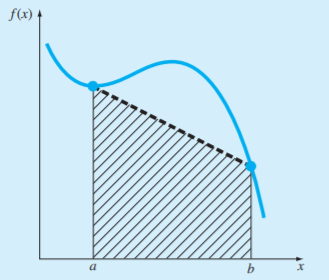
\includegraphics[width = .7\textwidth]{figures/firstO}
	\end{figure}
\end{frame}

\begin{frame}
	\frametitle{2nd order approximate}
	\begin{figure}
		\centering
		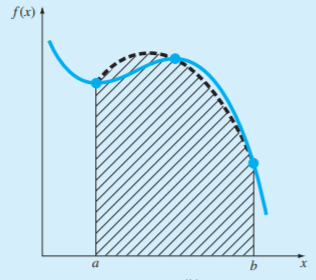
\includegraphics[width = .7\textwidth]{figures/secondO}
	\end{figure}
\end{frame}

\begin{frame}
	\frametitle{Piecewise function approximate}
	\begin{figure}
		\centering
		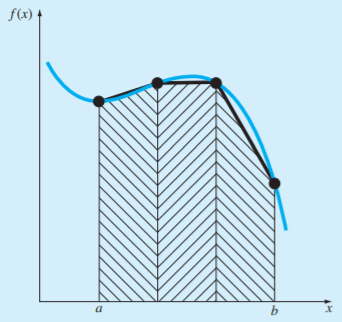
\includegraphics[width = .7\textwidth]{figures/Pieceise}
	\end{figure}
\end{frame}


\begin{frame}[t]
	\frametitle{Newton-Cotes formulas}
	Newton-Cotes formulas exist in 2 categories: \textit{closed forms} or \textit{open forms}. \\\vspace{10pt}
	\begin{minipage}{0.5\textwidth}
		The \textit{closed forms}
		are those where the data points at the beginning and end of the limits of integration are
		known \\\vspace{40pt}
		
		The \textit{open forms} have integration limits that extend beyond the range of the data 
	\end{minipage}
	\begin{minipage}{0.5\textwidth}
		\begin{figure}
			\centering
			\\\vspace{5pt}
			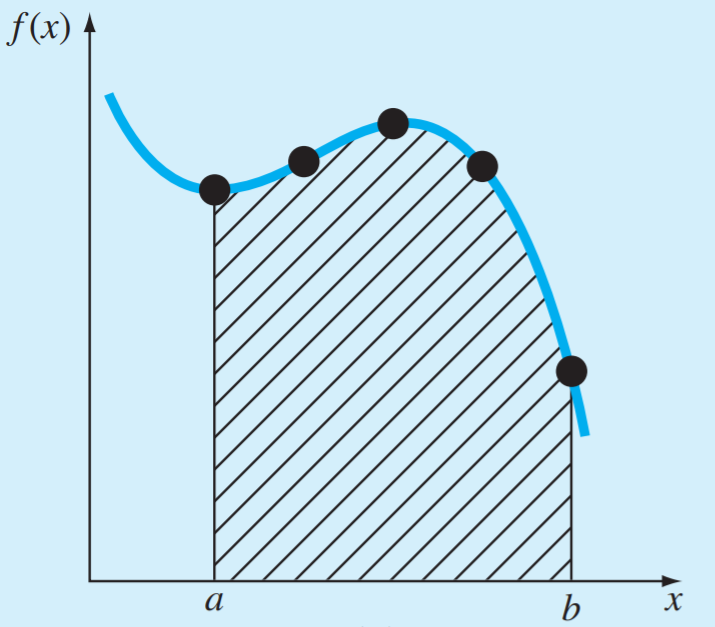
\includegraphics[width=.55\textwidth]{figures/closed}\\\vspace{5pt}
			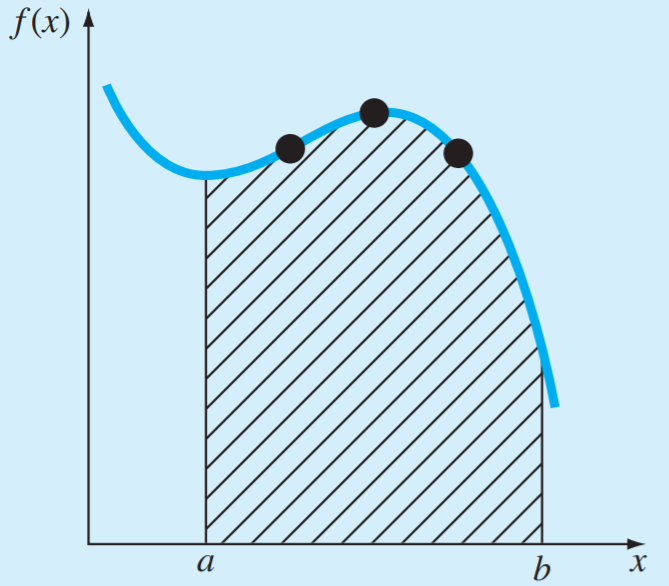
\includegraphics[width=.55\textwidth]{figures/open}
		\end{figure}
	\end{minipage}	
\end{frame}

\section{The Trapezoidal Rule}
\begin{frame}
	\frametitle{The Trapezoidal Rule}
	The trapezoidal rule is the first of the Newton-Cotes closed integration formulas. It is formed using the first order polynomial of type:
	$$I = \int_{a}^{b}\left[f(a)+\frac{f(b)-f(a)}{b-a}(x-a)\right]dx$$
	which has the solution
	$$I = (b-a)\frac{f(a)+f(b)}{2}$$
	Which is called the \textit{trapezoid rule}.
\end{frame}

\begin{frame}
	\frametitle{The Trapezoidal Rule}
	Geometrically, the trapezoidal rule is equivalent to approximating the area of the trapezoid under the straight line connecting $f(a)$ and $f(b)$\\\vspace{10pt}
	\begin{minipage}{0.5\textwidth}
		.
	\end{minipage}
	\begin{minipage}{0.5\textwidth}
		\begin{figure}
			\centering
			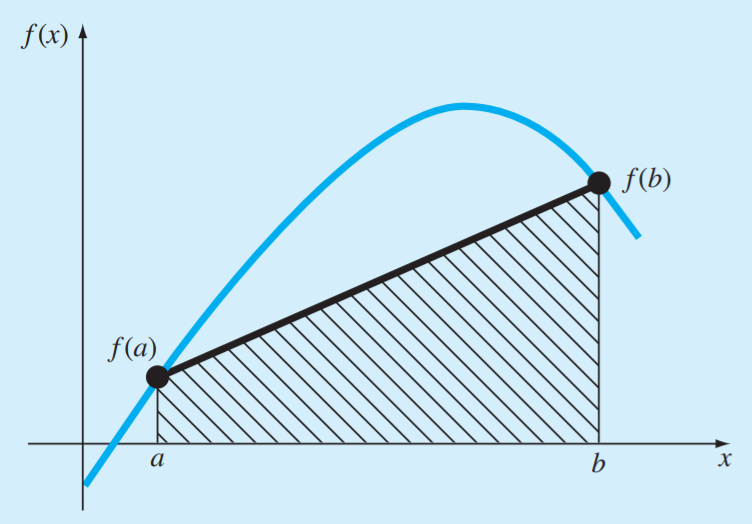
\includegraphics[width=0.75\textwidth]{figures/traprule}
		\end{figure}
	\end{minipage}
\end{frame}

\begin{frame}
	\frametitle{The Trapezoidal Rule}
	Geometrically, the trapezoidal rule is equivalent to approximating the area of the trapezoid under the straight line connecting $f(a)$ and $f(b)$\\\vspace{10pt}
	\begin{minipage}{0.5\textwidth}
		\begin{itemize}
			\item  Recall from geometry
			that the formula for computing the area of a trapezoid is the height times the average of the
			bases. 
		\end{itemize}
	\end{minipage}
	\begin{minipage}{0.5\textwidth}
	\begin{figure}
		\centering
		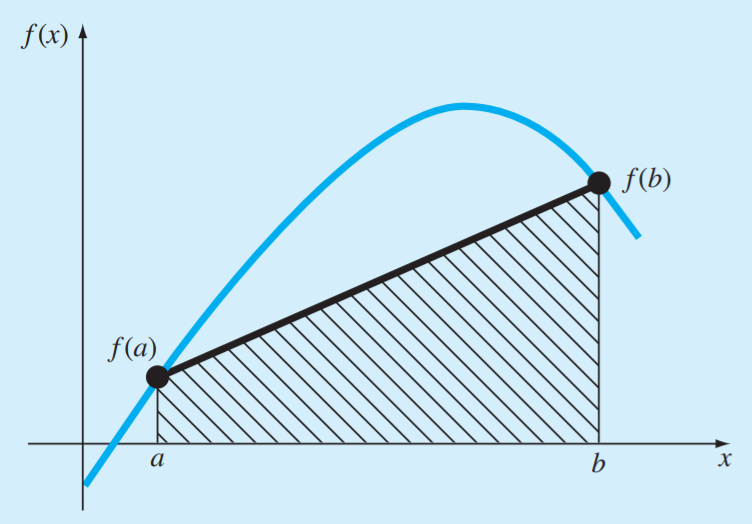
\includegraphics[width=0.9\textwidth]{figures/traprule}
	\end{figure}
    \end{minipage}
\end{frame}

\begin{frame}
	\frametitle{The Trapezoidal Rule}
	Geometrically, the trapezoidal rule is equivalent to approximating the area of the trapezoid under the straight line connecting $f(a)$ and $f(b)$\\\vspace{10pt}
	\begin{minipage}{0.5\textwidth}
		\begin{itemize}
			\item  Recall from geometry
			that the formula for computing the area of a trapezoid is the height times the average of the
			bases. 
			\item  In our case, the concept is the same but the trapezoid is on its side. Therefore, the
			integral estimate can be represented as
			$$I = \textrm{width } x \textrm{ average height}$$
		\end{itemize}
	\end{minipage}
	\begin{minipage}{0.5\textwidth}
		\begin{figure}
			\centering
			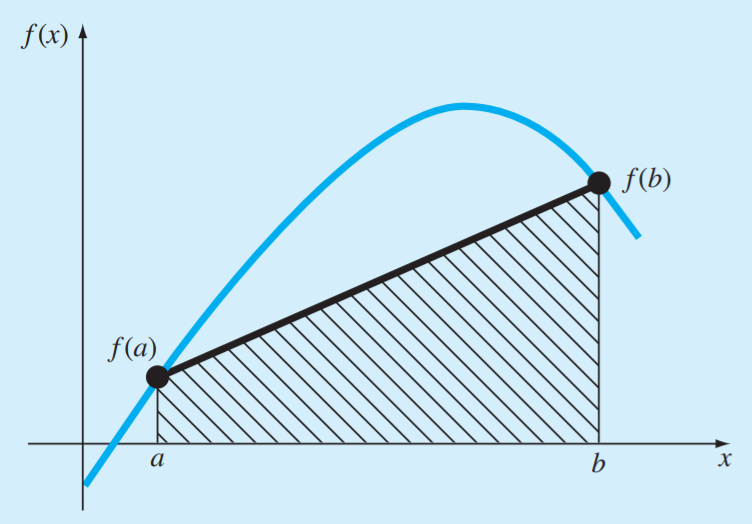
\includegraphics[width=0.9\textwidth]{figures/traprule}
		\end{figure}
	\end{minipage}
\end{frame}

\begin{frame}
	\frametitle{The Trapezoidal Rule}
	Geometrically, the trapezoidal rule is equivalent to approximating the area of the trapezoid under the straight line connecting $f(a)$ and $f(b)$\\\vspace{10pt}
	\begin{minipage}{0.5\textwidth}
		\begin{itemize}
			\item  Recall from geometry
			that the formula for computing the area of a trapezoid is the height times the average of the
			bases. 
			\item  In our case, the concept is the same but the trapezoid is on its side. Therefore, the
			integral estimate can be represented as
			$$I = \textrm{width } x \textrm{ average height}$$
			\item The width is $(b-a)$ and the average height is the average of the function values at
			the end points, or $\frac{[ f(a) + f(b)]}{2}$.
		\end{itemize}
	\end{minipage}
	\begin{minipage}{0.5\textwidth}
		\begin{figure}
			\centering
			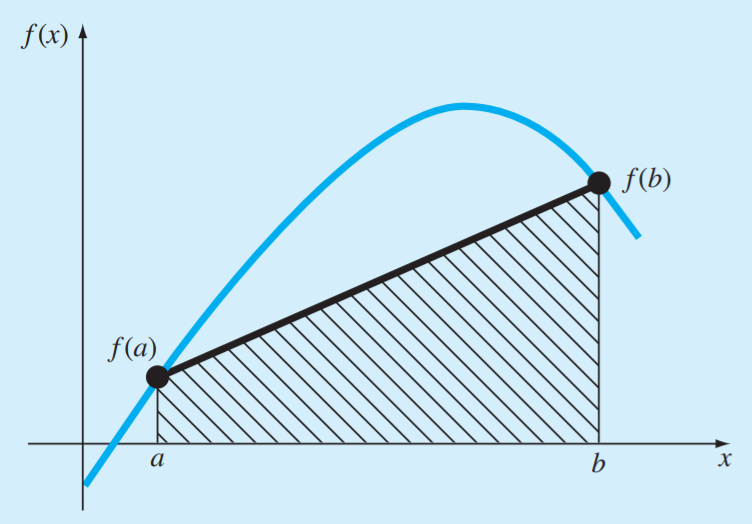
\includegraphics[width=0.9\textwidth]{figures/traprule}
		\end{figure}
	\end{minipage}
\end{frame}

\begin{frame}
	\frametitle{The Trapezoidal Rule}
	Geometrically, the trapezoidal rule is equivalent to approximating the area of the trapezoid under the straight line connecting $f(a)$ and $f(b)$\\\vspace{10pt}
	\begin{minipage}{0.5\textwidth}
		\begin{itemize}
			\item  Recall from geometry
			that the formula for computing the area of a trapezoid is the height times the average of the
			bases. 
			\item  In our case, the concept is the same but the trapezoid is on its side. Therefore, the
			integral estimate can be represented as
			$$I = \textrm{width } x \textrm{ average height}$$
			\item The width is $(b-a)$ and the average height is the average of the function values at
			the end points, or $\frac{[ f(a) + f(b)]}{2}$.\\\vspace{3pt}
		\end{itemize}
	\end{minipage}
	\begin{minipage}{0.5\textwidth}
		\begin{figure}
			\centering
			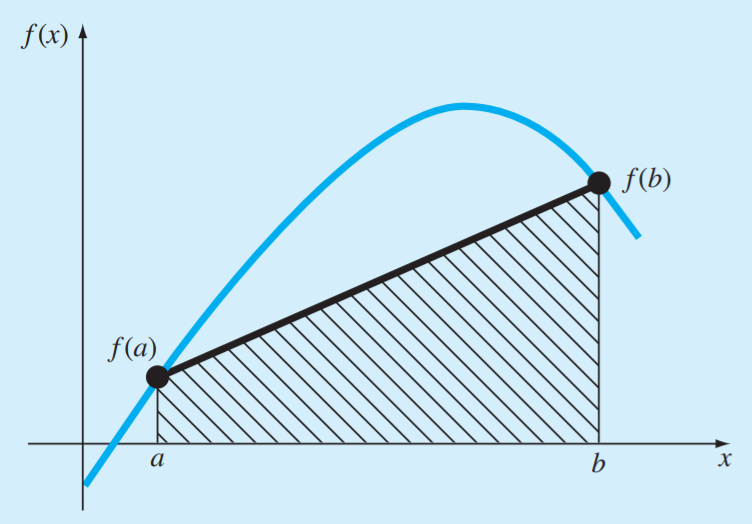
\includegraphics[width=0.9\textwidth]{figures/traprule}
		\end{figure}
	\end{minipage}
After substituting these values into the above equation, we get the trapezoid rule
$$I = (b-a)\frac{f(a)+f(b)}{2}$$

\end{frame}

\begin{frame}
	\frametitle{Error of the Trapezoidal Rule}
	When we employ the integral under a straight-line segment to approximate the integral
	under a curve, we obviously can incur an error that may be substantial 
	\begin{figure}
		\centering
		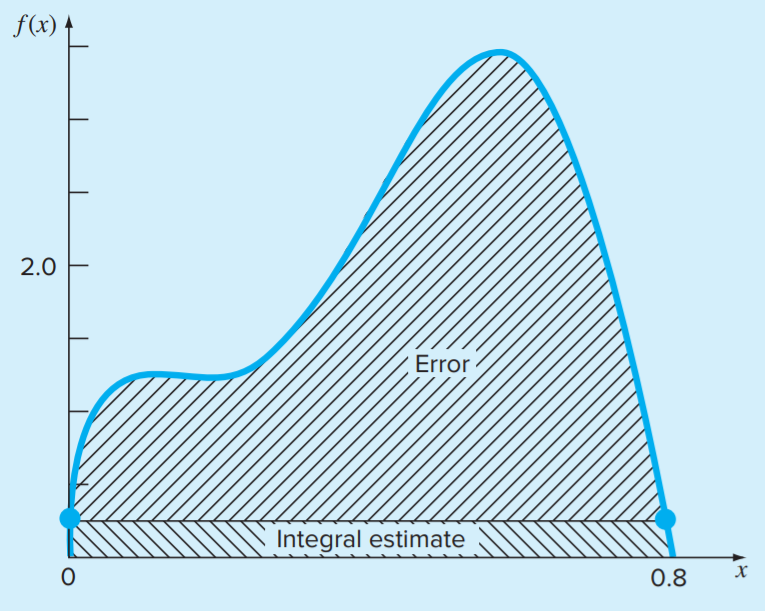
\includegraphics[width=0.7\textwidth]{figures/error}
	\end{figure}
\end{frame}

\begin{frame}
	\frametitle{Error of the Trapezoidal Rule}
	The type of error we will compute for this method is \textit{local truncation error}. The local truncation error is the amount error caused by one iteration of the method.\\\vspace{10pt}
	
	An estimate for the local truncation error for the trapezoid rule is 
	$$E_t =-\frac{1}{12}f''(\xi)(b-a)^3$$
	Where $\xi$ lies somewhere in the domain $[a,b]$. \\\vspace{10pt} 
\end{frame}

\begin{frame}
	\frametitle{Single Application of the Trapezoidal Rule}
	Let's use the trapezoid rule to numerically integrate
	$$f(x) =0.2+25x-200x^2+675x^3-900x^4+400x^5$$
	from $a = 0$ to $b=0.8$
\end{frame}

\begin{frame}
	\frametitle{Single Application of the Trapezoidal Rule}
	Let's use the trapezoid rule to numerically integrate
	$$f(x) =0.2+25x-200x^2+675x^3-900x^4+400x^5$$
	from $a = 0$ to $b=0.8$
	Recalling our formula for the trapezoid rule
	$$I = (b-a)\frac{f(a)+f(b)}{2}$$
	We can plug in the values for $f(0) = 0.2$
	and $f(0,8) = 0.232$
	$$I = (0.8-0)\frac{0.2+0.232}{2} = 0.1728$$
	
\end{frame}

\begin{frame}
	\frametitle{Single Application of the Trapezoidal Rule}
	Let's use the trapezoid rule to numerically integrate
	$$f(x) =0.2+25x-200x^2+675x^3-900x^4+400x^5$$
	from $a = 0$ to $b=0.8$
	Recalling our formula for the trapezoid rule
	$$I = (b-a)\frac{f(a)+f(b)}{2}$$
	We can plug in the values for $f(0) = 0.2$
	and $f(0,8) = 0.232$
	$$I = (0.8-0)\frac{0.2+0.232}{2} = 0.1728$$
	Now, we can find this integral analytically, it has an exact value of 1.640533. We can compute the percent relative error
	$$\epsilon_a = \frac{1.640533-0.1728}{1.640533} = 89.5\%$$ 
\end{frame}

\begin{frame}
	\frametitle{Single Application of the Trapezoidal Rule}
	Since we won't always know what the true solution is, we need to estimate the approximate error. We can do this using the local truncation error
	$$E_t =-\frac{1}{12}f''(\xi)(b-a)^3$$
\end{frame}

\begin{frame}
	\frametitle{Single Application of the Trapezoidal Rule}
	Since we won't always know what the true solution is, we need to estimate the approximate error. We can do this using the local truncation error
	$$E_t =-\frac{1}{12}f''(\xi)(b-a)^3$$
	The function's second derivative can be found analytically
	$$f''(x) = -400+4050x-10800x^2+8000x^3$$
\end{frame}

\begin{frame}
	\frametitle{Single Application of the Trapezoidal Rule}
	Since we won't always know what the true solution is, we need to estimate the approximate error. We can do this using the local truncation error
	$$E_t =-\frac{1}{12}f''(\xi)(b-a)^3$$
	The function's second derivative can be found analytically
	$$f''(x) = -400+4050x-10800x^2+8000x^3$$
	To find $f''(\xi)$, we will take the average value of the second derivative which is computed as
	$$ \bar{f}''(x) = \frac{\int_{0}^{0.8}(-400+4050x-10800x^2+8000x^3)dx}{0.8-0} = -60$$
	
\end{frame}

\begin{frame}
	\frametitle{Single Application of the Trapezoidal Rule}
	Since we won't always know what the true solution is, we need to estimate the approximate error. We can do this using the local truncation error
	$$E_t =-\frac{1}{12}f''(\xi)(b-a)^3$$
	The function's second derivative can be found analytically
	$$f''(x) = -400+4050x-10800x^2+8000x^3$$
	To find $f''(\xi)$, we will take the average value of the second derivative which is computed as
	$$ \bar{f}''(x) = \frac{\int_{0}^{0.8}(-400+4050x-10800x^2+8000x^3)dx}{0.8-0} = -60$$
	Which we can now substitute into our truncation error equation
	$$E_a = -\frac{1}{12}(-60)(0.8^3) = 2.56$$
	
\end{frame}

\begin{frame}
	\frametitle{Single Application of the Trapezoidal Rule}
	Since we won't always know what the true solution is, we need to estimate the approximate error. We can do this using the local truncation error
	$$E_t =-\frac{1}{12}f''(\xi)(b-a)^3$$
	The function's second derivative can be found analytically
	$$f''(x) = -400+4050x-10800x^2+8000x^3$$
	To find $f''(\xi)$, we will take the average value of the second derivative which is computed as
	$$ \bar{f}''(x) = \frac{\int_{0}^{0.8}(-400+4050x-10800x^2+8000x^3)dx}{0.8-0} = -60$$
	Which we can now substitute into our truncation error equation
	$$E_a = -\frac{1}{12}(-60)(0.8^3) = 2.56$$
	You may have noticed we changed the $E_t$ to $E_a$, this is because for an interval of this size, the average second derivative is not necessarily an accurate approximation of $f''(\xi)$. We are denoting that this is an approximation using the subscript a. 
\end{frame}

\begin{frame}
	\frametitle{The Composite Trapezoid Rule}
	One way to improve the accuracy of the trapezoidal rule is to divide the integration interval from $a$ to $b$ into a number of segments and apply the method to each segment.\\\vspace{10pt}
	\begin{minipage}{0.5\textwidth}
		.
	\end{minipage}
	\begin{minipage}{0.5\textwidth}
		\begin{figure}
			\centering
			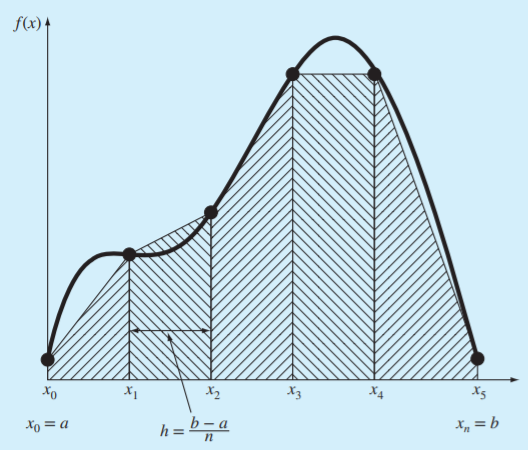
\includegraphics[width=0.8\textwidth]{figures/compositeTrap}
		\end{figure}
	\end{minipage}
\end{frame}

\begin{frame}
	\frametitle{The Composite Trapezoid Rule}
	One way to improve the accuracy of the trapezoidal rule is to divide the integration interval from $a$ to $b$ into a number of segments and apply the method to each segment.\\\vspace{10pt}
	\begin{minipage}{0.5\textwidth}
	 The areas of individual segments can then be added to yield the integral for the entire interval.\\\vspace{4pt}

	\end{minipage}
	\begin{minipage}{0.5\textwidth}
		\begin{figure}
			\centering
			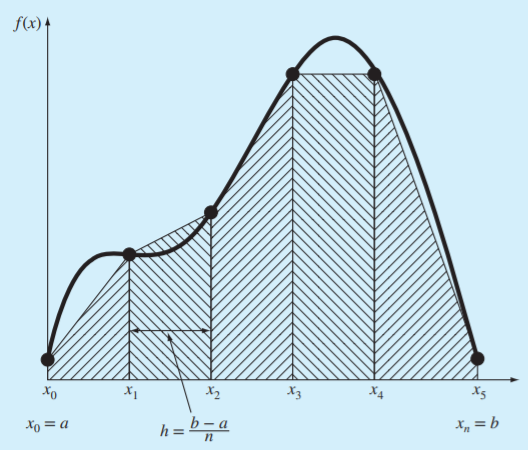
\includegraphics[width=0.8\textwidth]{figures/compositeTrap}
		\end{figure}
	\end{minipage}
\end{frame}

\begin{frame}
	\frametitle{The Composite Trapezoid Rule}
	One way to improve the accuracy of the trapezoidal rule is to divide the integration interval from $a$ to $b$ into a number of segments and apply the method to each segment.\\\vspace{10pt}
	\begin{minipage}{0.5\textwidth}
		The areas of individual segments can then be added to yield the integral for the entire interval.\\\vspace{4pt}
		
		There are $n+1$ equally spaced base points $(x_0,x_1,x_2,...,x_n)$ with $n$ segments of equal width:
		$$h = \frac{b-a}{n}$$
		In this figure $n = 5$
	\end{minipage}
	\begin{minipage}{0.5\textwidth}
		\begin{figure}
			\centering
			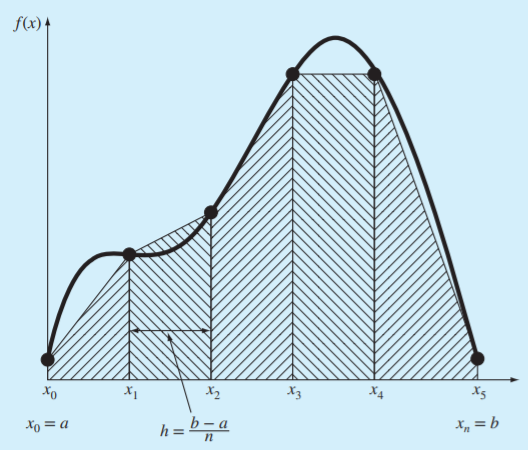
\includegraphics[width=0.8\textwidth]{figures/compositeTrap}
		\end{figure}
	\end{minipage}
\end{frame}

\begin{frame}
	\frametitle{The Composite Trapezoid Rule}
	One way to improve the accuracy of the trapezoidal rule is to divide the integration interval from $a$ to $b$ into a number of segments and apply the method to each segment.\\\vspace{10pt}
	\begin{minipage}{0.5\textwidth}
		The areas of individual segments can then be added to yield the integral for the entire interval.\\\vspace{4pt}
		
		There are $n+1$ equally spaced base points $(x_0,x_1,x_2,...,x_n)$ with $n$ segments of equal width:
		$$h = \frac{b-a}{n}$$
		In this figure $n = 5$ \\\vspace{4pt}
	\end{minipage}
	\begin{minipage}{0.5\textwidth}
		\begin{figure}
			\centering
			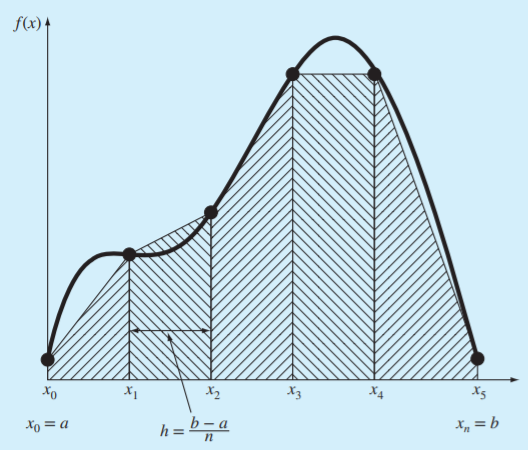
\includegraphics[width=0.8\textwidth]{figures/compositeTrap}
		\end{figure}
	\end{minipage}

If $a = x_0$ and $b=x_n$, the total integration can be represented by
$$ I = \int_{x_0}^{x_1}f(x)dx + \int_{x_1}^{x_2}f(x)dx + ... + \int_{x_{n-1}}^{x_n}f(x)dx$$
\end{frame}

\begin{frame}
	\frametitle{The Composite Trapezoid Rule}
	If $a = x_0$ and $b=x_n$, the total integration can be represented by
	$$ I = \int_{x_0}^{x_1}f(x)dx + \int_{x_1}^{x_2}f(x)dx + ... + \int_{x_{n-1}}^{x_n}f(x)dx$$
	Substituting the trapezoidal rule for each integral yields
	$$I = h\frac{f(x_0)+f(x_1)}{2}+h\frac{f(x_1)+f(x_2)}{2}+...+h\frac{f(x_{n-1})+f(x_n)}{2}$$
\end{frame}

\begin{frame}
	\frametitle{The Composite Trapezoid Rule}
	If $a = x_0$ and $b=x_n$, the total integration can be represented by
	$$ I = \int_{x_0}^{x_1}f(x)dx + \int_{x_1}^{x_2}f(x)dx + ... + \int_{x_{n-1}}^{x_n}f(x)dx$$
	Substituting the trapezoidal rule for each integral yields
	$$I = h\frac{f(x_0)+f(x_1)}{2}+h\frac{f(x_1)+f(x_2)}{2}+...+h\frac{f(x_{n-1})+f(x_n)}{2}$$
	Which can be re-written as
	$$ I = \frac{h}{2}\left[f(x_0)+2\sum_{i=1}^{n-1}f(x_i)+f(x_n)\right]$$
\end{frame}

\begin{frame}
	\frametitle{Error of the The Composite Trapezoid Rule}
	An error for the composite trapezoidal rule can be obtained by summing the individual
	errors for each segment to give
	$$ E_t = -\frac{(b-a)^3}{12n^3}\sum_{i+1}^{n}f''(\xi_i)$$
	
\end{frame}

\begin{frame}
	\frametitle{Error of the The Composite Trapezoid Rule}
	An error for the composite trapezoidal rule can be obtained by summing the individual
	errors for each segment to give
	$$ E_t = -\frac{(b-a)^3}{12n^3}\sum_{i+1}^{n}f''(\xi_i)$$
	Where $f''(x_i)$ is the second derivative at a point $\xi$ located in segment $i$. This result can be simplified by estimating the mean or average value of the second derivative for the entire interval as
	$$\bar{f}''\cong \frac{\sum_{i=1}^{n}f''(\xi_i)}{n} $$
	
\end{frame}

\begin{frame}
	\frametitle{Error of the The Composite Trapezoid Rule}
	An error for the composite trapezoidal rule can be obtained by summing the individual
	errors for each segment to give
	$$ E_t = -\frac{(b-a)^3}{12n^3}\sum_{i+1}^{n}f''(\xi_i)$$
	Where $f''(x_i)$ is the second derivative at a point $\xi$ located in segment $i$. This result can be simplified by estimating the mean or average value of the second derivative for the entire interval as
	$$\bar{f}''\cong \frac{\sum_{i=1}^{n}f''(\xi_i)}{n} $$
	Subbing this into our equation for $E_t$, we can approximate the error $E_a$
	$$E_a = -\frac{(b-a)^3}{12n^2}\bar{f}''$$
	Where $\bar{f}''$ is found the same was as in the case of the single application of the trapezoidal rule.
\end{frame}

\begin{frame}
	\frametitle{Composite Trapezoidal Rule Example}
	Looking back at our previous problem, let's use the composite trapezoid rule to numerically integrate
	$$f(x) =0.2+25x-200x^2+675x^3-900x^4+400x^5$$
	from $a = 0$ to $b=0.8$ with $n = 2$. Recalling our formula for the composite trapezoidal rule:
	$$I = h\frac{f(x_0)+f(x_1)}{2}+h\frac{f(x_1)+f(x_2)}{2}+...+h\frac{f(x_{n-1})+f(x_n)}{2}$$
	
\end{frame}

\begin{frame}
	\frametitle{Composite Trapezoidal Rule Example}
	Looking back at our previous problem, let's use the composite trapezoid rule to numerically integrate
	$$f(x) =0.2+25x-200x^2+675x^3-900x^4+400x^5$$
	from $a = 0$ to $b=0.8$ with $n = 2$. Recalling our formula for the composite trapezoidal rule:
	$$I = h\frac{f(x_0)+f(x_1)}{2}+h\frac{f(x_1)+f(x_2)}{2}+...+h\frac{f(x_{n-1})+f(x_n)}{2}$$
	In this case, 
	$$I = h\frac{f(x_0)+f(x_1)}{2}+h\frac{f(x_1)+f(x_2)}{2}$$
\end{frame}

\begin{frame}
	\frametitle{Composite Trapezoidal Rule Example}
	Looking back at our previous problem, let's use the composite trapezoid rule to numerically integrate
	$$f(x) =0.2+25x-200x^2+675x^3-900x^4+400x^5$$
	from $a = 0$ to $b=0.8$ with $n = 2$. Recalling our formula for the composite trapezoidal rule:
	$$I = h\frac{f(x_0)+f(x_1)}{2}+h\frac{f(x_1)+f(x_2)}{2}+...+h\frac{f(x_{n-1})+f(x_n)}{2}$$
	In this case, 
	$$I = h\frac{f(x_0)+f(x_1)}{2}+h\frac{f(x_1)+f(x_2)}{2}$$
	Where 
	$$h = \frac{b-a}{n} = \frac{0.8-0}{2} = 0.4$$
\end{frame}

\begin{frame}
	\frametitle{Composite Trapezoidal Rule Example}
	Looking back at our previous problem, let's use the composite trapezoid rule to numerically integrate
	$$f(x) =0.2+25x-200x^2+675x^3-900x^4+400x^5$$
	from $a = 0$ to $b=0.8$ with $n = 2$. Recalling our formula for the composite trapezoidal rule:
	$$I = h\frac{f(x_0)+f(x_1)}{2}+h\frac{f(x_1)+f(x_2)}{2}+...+h\frac{f(x_{n-1})+f(x_n)}{2}$$
	In this case, 
	$$I = h\frac{f(x_0)+f(x_1)}{2}+h\frac{f(x_1)+f(x_2)}{2}$$
	Where 
	$$h = \frac{b-a}{n} = \frac{0.8-0}{2} = 0.4$$
	Therefore,
	$$ x_0 = 0, \quad x_1 = 0.4, \quad x_2 = 0.8$$.
\end{frame}

\begin{frame}
	\frametitle{Composite Trapezoidal Rule Example}
	Looking back at our previous problem, let's use the composite trapezoid rule to numerically integrate
	$$f(x) =0.2+25x-200x^2+675x^3-900x^4+400x^5$$
	from $a = 0$ to $b=0.8$ with $n = 2$. Recalling our formula for the composite trapezoidal rule:
	$$I = h\frac{f(x_0)+f(x_1)}{2}+h\frac{f(x_1)+f(x_2)}{2}+...+h\frac{f(x_{n-1})+f(x_n)}{2}$$
	In this case, 
	$$I = h\frac{f(x_0)+f(x_1)}{2}+h\frac{f(x_1)+f(x_2)}{2}$$
	Where 
	$$h = \frac{b-a}{n} = \frac{0.8-0}{2} = 0.4$$
	Therefore,
	$$ x_0 = 0, \quad x_1 = 0.4, \quad x_2 = 0.8$$.
	$$f(0) = 0.2, \quad f(0.4) = 2.456, \quad f(0.8) = 0.232$$
\end{frame}

\begin{frame}
	\frametitle{Composite Trapezoidal Rule Example}
	Looking back at our previous problem, let's use the composite trapezoid rule to numerically integrate
	$$f(x) =0.2+25x-200x^2+675x^3-900x^4+400x^5$$
	from $a = 0$ to $b=0.8$ with $n = 2$. Recalling our formula for the composite trapezoidal rule:
	$$I = h\frac{f(x_0)+f(x_1)}{2}+h\frac{f(x_1)+f(x_2)}{2}+...+h\frac{f(x_{n-1})+f(x_n)}{2}$$
	In this case, 
	$$I = h\frac{f(x_0)+f(x_1)}{2}+h\frac{f(x_1)+f(x_2)}{2}$$
	Where 
	$$h = \frac{b-a}{n} = \frac{0.8-0}{2} = 0.4$$
	Therefore,
	$$ x_0 = 0, \quad x_1 = 0.4, \quad x_2 = 0.8$$.
	$$f(0) = 0.2, \quad f(0.4) = 2.456, \quad f(0.8) = 0.232$$
	Substituting these into our equation for $I$
	$$ I = 0.4\frac{0.2+2.456}{2}+0.4\frac{2.456+0.232}{2} = 1.0688$$
\end{frame}

\begin{frame}
	\frametitle{Composite Trapezoidal Rule Example}
	We can use the average second derivate from the single application of the trapezoidal rule
	$$\bar{f}''\cong -60 $$
	Therefore, our error is 
	$$E_a = -\frac{0.8^3}{12(2)^2}(-60) =0.64$$
	Which is a quarter of the error we found using a single application of the trapezoidal rule.
\end{frame}

\begin{frame}
	\frametitle{Composite Trapezoidal Rule Example}
	We can use the average second derivate from the single application of the trapezoidal rule
	$$\bar{f}''\cong -60 $$
	Therefore, our error is 
	$$E_a = -\frac{0.8^3}{12(2)^2}(-60) =0.64$$
	Which is a quarter of the error we found using a single application of the trapezoidal rule. \\\vspace{10pt}
	
	This is because the error is inversly related to the square of $n$, so as we double n, we quarter the error.
\end{frame}

\begin{frame}
	\frametitle{Composite Trapezoid Rule Pseudocode}
	How would you code the composite trapezoid rule? Write your pseudocode and submit it to the canvas discussion board \textbf{Composite Trapezoidal Rule}. \\\vspace{10pt}
	
	NOTE: Unlike the other methods we have covered, this one does not need a cut-off condition. This code is looping over the sections of your interval to find the total area under the curve. In other words, you don't need to factor in error.
\end{frame}	

\end{document}
